%%%%%%%%%%%%%%%%%%%%%%%%%%%%%%%%%%%%%%%%%
% University/School Laboratory Report
% LaTeX Template
% Version 3.1 (25/3/14)
%
% This template has been downloaded from:
% http://www.LaTeXTemplates.com
%
% Original author:
% Linux and Unix Users Group at Virginia Tech Wiki 
% (https://vtluug.org/wiki/Example_LaTeX_chem_lab_report)
%
% License:
% CC BY-NC-SA 3.0 (http://creativecommons.org/licenses/by-nc-sa/3.0/)
%
%%%%%%%%%%%%%%%%%%%%%%%%%%%%%%%%%%%%%%%%%

%----------------------------------------------------------------------------------------
%	PACKAGES AND DOCUMENT CONFIGURATIONS
%----------------------------------------------------------------------------------------

\documentclass{article}

\usepackage{graphicx} % Required for the inclusion of images
\graphicspath{ {images/} } % path for images
\usepackage{subcaption} % placing multiple images on one by one in a line
\usepackage{wrapfig} % placing an image along with text in a line
\usepackage{natbib} % Required to change bibliography style to APA
\usepackage{amsmath} % Required for some math elements 
\usepackage{enumerate} % use enumarated lists
\usepackage{svg}	% include *.svg graphical file forma
\usepackage{pgfplots} % to plot a function

\setlength\parindent{0pt} % Removes all indentation from paragraphs

\renewcommand{\labelenumi}{\alph{enumi}.} % Make numbering in the enumerate environment by letter rather than number (e.g. section 6)

\usepackage{times} % Uncomment to use the Times New Roman font

%----------------------------------------------------------------------------------------
%	DOCUMENT INFORMATION
%----------------------------------------------------------------------------------------

\title{Lab Project: Computer Graphics \\ Building a basic ray tracer \\ SS2017} % Title

\author{Haralambi \textsc{Todorov}} % Author name

\date{\today} % Date for the report

\begin{document}

\maketitle % Insert the title, author and date

\begin{center}
\begin{tabular}{l r}
Advisor: & Prof. Dr.-Ing. Matthias Teschner % Instructor/supervisor
\end{tabular}
\end{center}

% If you wish to include an abstract, uncomment the lines below
% \begin{abstract}
% Abstract text
% \end{abstract}

%----------------------------------------------------------------------------------------
%	SECTION 1
%----------------------------------------------------------------------------------------

\section{Introduction}
\label{sec:intro}
The main objective of the \textit{Lab project: Computer Graphics} was to make the author familiar with the basic concepts of a ray tracer through the implementation of one. This lab report aims to present the gathered knowledge.

% explain the structure of the current lab report
\subsection{Report overview}
The report is split into five chapters with, each explaining a certain part of the implemented ray tracer. The ordering of the chapters tries to follow the implementation order the author followed during the project. 

\vspace*{\baselineskip}

Current chapter (\ref{sec:intro}) is an introductory one giving details about the organisation of this report, motivation about why is ray tracing an important rendering technique and where does it find application nowadays, along with some information on the roots of ray tracing, the basic idea of the ray tracing algorithm and some implementation notes regarding the accompanying ray tracer.

\vspace*{\baselineskip}

Chapter (\ref{sec:isects}) deals with one of the fundamental parts of a ray tracer, the ray-object intersection test. It starts with the geometric definition of a half-line (ray), goes on with the different type of geometries the ray tracer supports (spheres, triangles, axis-aligned boxes and triangulated meshes) and how the half-line intersects with these geometries.

\vspace*{\baselineskip}

Chapter (\ref{sec:cameras}) is concerned with how the camera and the image plane are modelled in the ray tracer. It explains how the image plane is mapped within the 3D scene and the two supported camera projections - orthographic and perspective, along with their configurable parameters. The chapter goes on with why is aliasing perceived by the viewer and how can one reduce it by using the half-jittered sampling technique. It finishes with the use of gamma correction to enhance the visual appearance of the generated images. 

\vspace*{\baselineskip}

Chapter (\ref{sec:shading}) deals with the shading of objects rendered in a scene. It begins by explaining how light sources are modeled, goes on with the concept behind the Phong illumination model and the physical motivation behind its components, how shadows are ray traced and lastly, it presents reflective and refractive materials and how these types of materials are ray traced.

\vspace*{\baselineskip}

Chapter (\ref{sec:transform}) deals with transformations, explaining the motivation behind the use of homogeneous notation, the different type of supported transformations on objects, light sources and cameras and why the inverse view transformation is useful in a ray tracer.

\vspace*{\baselineskip}

Chapter (\ref{sec:accel}) is concerned with how one can reduce the computation time per generated image. 
% Firstly, it explains the concept behind axis-aligned bounding boxes and the benefits they bring, followed by a more advanced acceleration method, the uniform grid.

% why should one bother to implement a ray tracer
\subsection{Why is ray tracing important}
Ray tracing is one of the rendering techniques capable of producing images with a high degree of visual realism. It can naturally incorporate physically based visual effects such as reflections, refractions, caustics, soft shadows and others. This advantage makes the technique very attractive to movie and commercial studios, automotive industry (see figure \ref{fig:audi}), as well as architectural design studios (see figure \ref{fig:arch}) to simulate realistic illumination.  

\begin{figure}[h]
	\centering
	
	% show car image
	\begin{subfigure}{0.5\textwidth}
		\includegraphics[width=0.9\textwidth]{audi}
		\caption{"Another R8" by Filip Sadlon \\ rendered using Blender Render}
		\label{fig:audi}
	\end{subfigure}%
	\hfill
	\begin{subfigure}{0.5\textwidth}
		\includegraphics[width=0.9\textwidth]{archi_render}
		\caption{"Mies Van Der Rohe Farnsworth House" by Alessandro Prodan using Mental Ray}
		\label{fig:arch}
	\end{subfigure}
	
	\caption{Ray tracing used for visualisations by different industries}
\end{figure}

Although one can produce very stunning imagery with a ray tracing based render engine, this  comes at a great computational cost, e.g.\ a frame from a present-day computer generated movie by Pixar takes between three and eight hours to render. \cite{pixarRentime} \\
Despite great computation times, major animation studios seem nowadays to be fond of ray tracing and switch to ray tracing from scanline-based rendering approaches, such as "REYES", which have been proved stable and fast over the years to ray tracing. \cite{pixarSwitch} That points to the demands in the entertainment industry for more physically accurate imagery, but also pushes the boundaries of research in ray tracing and its computational efficiency. \cite{disneyHyperion}

% some history behind ray tracing
\subsection{The roots of ray tracing}
The first ray tracing algorithm was introduced by Arthur Appel in 1968 \cite{appel}, whose idea was to shoot rays from the eye (camera), one per pixel, and find the closest object blocking the path of that ray. Using the material properties and the effect of the lights in the scene, this algorithm can determine the shading of objects. \\
The next notable contribution in ray tracing was made by Turner Whitted in 1979 \cite{whitted}, who introduced a technique to compute shadows, as well as the idea of recursive ray tracing to handle reflective and refractive materials. (see figure \ref{fig:whitted_example}).  

Other major contributions in the scene of ray tracing were made by Robert Cook in 1984 \cite{cook} and James Kajiya in 1986 \citep{kajiya}, introducing distributed ray tracing and the Rendering equation respectively. Because the accompanying ray tracer does not make extensive use of these concepts, they won't be discussed in detail.

% show whitted like image
\begin{figure}[h]
	\centering
    \includegraphics[width=0.8\textwidth]{whitted_example}
    \caption{A Whitted-like scene with reflective (back) and refractive (front left) spheres rendered in the accompanying ray tracer}
    \label{fig:whitted_example}
\end{figure}

% basic ray tracing algorithm concept
\subsection{Basics of the ray tracing algorithm}
For the following explanation we make the assumption we have a camera with perspective projection. The algorithm then works by tracing a path from an imaginary eye (camera) through each pixel in a virtual image plane (in front of the camera) and calculating the radiance of the object visible through it.

Typically, each ray must be tested for intersection with some subset of all the objects in the scene. Once the nearest object has been identified, the algorithm will estimate the incoming light at the point of intersection, examine the material properties of the object, and combine this information to calculate the final color of the pixel (see figure \ref{fig:concept}). 

% show image depicting basic ray tracing algorithm
\begin{figure}[h]
	\centering
    \includegraphics[width=0.6\textwidth]{ray_trace_algo}
	\caption{Image depicting the concept behind the ray tracing algorithm. Wikipedia}
    \label{fig:concept}
\end{figure}

\subsection{Implementation notes}

% details on the OS and the programming environment
The accompanying ray tracer is developed under \textit{macOS Sierra (version 10.12)} in the \textit{C++} programming language using the ``\textit{Apple LLVM version 8.1.0 (clang-802.0.42)}'' compiler. The choice of the programming language was based on the adivise of Prof. Dr.-Ing. Matthias Teschner, as well as on the suggestion of many renowned authors, who teach ray tracing, such as Peter Shirley \cite{realisticRaytracing} and Kevin G. Suffern \cite{rftgu}. Another fact worth mentioning is that many \textit{state of the art} ray tracers are implemented \textit{C++} such as Pixar's \textit{RenderMan}  and Solid Angle's \textit{Arnold}.

\vspace*{\baselineskip}

% list of external libraries
The author makes use of following external libraries:
\begin{itemize}
	\itemsep0em 	% reduce space between list items
	\item \textit{OpenGL Mathematics (glm)}: a header only C++ mathematics library for graphics software. The library is used to provide robust implementation for manipulations on matrices and vectors.
	\item \textit{png++}: a C++ wrapper for libpng library. The library is used to save rendered images into \textit{*.png} graphics file format. 
\end{itemize}

\vspace*{\baselineskip}

% details on the code structure
The actual ray tracer's source code, inside the`` \textit{src}'' folder, is split into multiple files. One can structure it into seven principal elements, some of which also include derivations. Each of them will be discussed in detail in the following chapters. The following is a high-level overview of the structure:
\begin{itemize}
	\itemsep0em 	% reduce space between list items
	
	\item \textit{Camera} (see ch. \ref{sec:cameras}): The camera consists of one base class \textbf{Camera} and its two derived classes - the supported camera projections \textbf{orthographic} and \textbf{perspective}. There are described the procedures on how to create a Camera object with a given projection and its desired parameters, how to move it in world space (by applying transformations) and how to render an image using the encoded camera configuration. There is also the procedure on how to apply a view transformation on the objects and light sources in a scene.

	\item \textit{ImagePlane} (see ch. \ref{sec:cameras}): The image plane class converts a frame buffer object into one of the supported graphics file formats (\textit{*.png} or \textit{*.ppm}). During the conversion process it encodes a gamma correction on the saved image file. 
	
	\item \textit{Light} (see ch. \ref{sec:shading}): The light consists of one base class \textbf{Light} and its two derived classes - the supported light types \textbf{directional} and \textbf{point}. There are described the procedures on how to create a light source object by given type and parameters, how to move it in world space (by applying transformations) and how it illuminates a surface point.
	
	\item \textit{Object} (see ch. \ref{sec:isects}): The object consists of one base class \textbf{Object} and its three derived classes - the supported object types \textbf{sphere}, \textbf{triangle} and \textbf{triangle mesh} as well a fourth object type \textbf{axis aligned bounding box}, which only serves to accelerate intersection tests and is not being shaded. There are described the procedures on how to create a object by given type and parameters, how to move it in world space (by applying transformations) and whether a given ray intersects this object, and if yes, at which surface point of the object.
	
	\item \textit{Ray} (see ch. \ref{sec:isects}): The ray class describes the procedure of creating a half line object with given parameters in world space and how to trace it within a scene. 
	
	\item \textit{Utilities}: In the \textbf{utilities} header file one stores constants and definitions of structures, which are used on multiple places within the project. 
	
	\item \textit{main}: The main file serves the purpose to describe a whole scene and to gather statistical informations about a given rendered scene. 
		
\end{itemize}

%----------------------------------------------------------------------------------------
%	SECTION 2
%----------------------------------------------------------------------------------------

\section{Ray-object intersection tests}
\label{sec:isects}
The main objective of the current chapter is to present the concepts along with some noteworthy mentioning implementation details about the ray-object intersection tests used in the ray tracer.

\vspace*{\baselineskip}

To explore ray-object intersections, one has to first define what is an intersection. An intersection is a point along a half-line (from now on one will use the word \textit{ray} meaning half-line) at which а given ray intersects certain object. Mostly one is interested in the nearest intersection point along a ray.

\subsection{Ray}

% how is a ray geometrically defined
A ray is geometrically defined using two vectors: a point $o$, which is called \textit{origin} and a normal vector $\hat{d}$, which is gives the \textit{direction} of the ray. In order to give the exact location of an intersection point $p$ along the ray, one introduces a scalar value $t$, which is the distance between the ray's origin $o$ and the intersection point $p$. One is mainly interested in intersection points "in front" of the ray, so $t$ should have positive values. The parametric equation for a point along a ray looks like: \cite{rftgu}

% intersection point along a ray
\begin{align}
	p(t) = o + t\hat{d}
	\label{eq:ray}
\end{align}

% components of the ray within the ray tracer
Within the implemented ray tracer a ray has five data members: 
\begin{itemize}
	\itemsep0em 	% reduce space between list items
	\item \textit{origin}
	\item \textit{direction}
	\item \textit{inverse of the ray's direction ($1 / \hat{d}$)}
	\item \textit{sign of the ray's direction}
	\item \textit{type component: \textbf{primary}, \textbf{shadow}, \textbf{reflection}, \textbf{refraction}}
\end{itemize}

\vspace*{\baselineskip}

The author has decided not to have an intersection point data member stored within the ray for memory efficiency. Depending on the scene a (big) part of the rays could not have any intersection points at all. \\
The \textit{inverse of the ray's direction} and \textit{sign of the ray's direction} data members are used to optimize the performance of the ray-axis-aligned bounding box intersection test. Details will be provided in the following section on the topic.\\
% types of a ray
The type component is used for distinguishing between different types of rays which are used to give statistic information on a rendered scene.

\subsection{Sphere}

% some motivation on why one can render spheres... easy to implement
% easy to intersect
In the following section one discusses how a sphere is being intersected by a ray. The method used by the  author is based on the geometric properties of a sphere.

\vspace*{\baselineskip}

% how is a sphere defined in the ray tracer
A sphere is defined by two components: a vector $c$, representing the sphere's center and a scalar value $r$, representing the sphere's radius. In the implemented ray tracer the author introduces a third component $r^2$ which is precomputed when constructing the sphere or when applying transformations which alter the sphere's radius. The parameter is later used to optimize the computation time of a ray-sphere intersection test.

% show ray-spere intersection graphic
% [11] is used to tell LaTeX the number of narrow lines; default is at 35... not good for every case
% see following link for detailed explanation: https://tex.stackexchange.com/questions/214532/how-to-end-wrapfigure-environment
\begin{wrapfigure}[10]{r}{0.5\textwidth} 
    \centering
    \includegraphics[width=0.4\textwidth]{ray_sphere}
    \caption{A graphical motivation for the ray-sphere intersection test}
    \label{fig:raysphere}
\end{wrapfigure}

% ray-sphere intersection
Figure \ref{fig:raysphere} is of graphical assistance for the algorithm's concept. The following notation is the same as on the figure. The goal of the algorithm is to compute the intersection point  if the point in front of the ray's origin $p(s-q)$, or if the ray's origin is inside the sphere $p(s+q)$. The algorithm can terminate beforehand, if it is sure that there is no intersection point for the given ray and sphere. The algorithm can be split in three parts: \cite{realtime_ren}

% explain the ray-sphere intersection test splitting it into 3 parts 
\begin{enumerate}[1.]
\item This part is concerned with determining if a sphere is behind the ray's origin. If that is the case, one don't need to do further calculations and can exit the procedure for ray-sphere intersection. To do so, first the vector $l = c - o$ and its squared length $l^2 = l \bullet l$ are computed. Further one computes the projection of $l$ onto the ray's direction $\hat{d}$, $s = l \cdot \hat{d}$. If $l^2 > r^2$, (the origin of the ray is outside the sphere) and $s < 0$ (ray's direction and the vector $l$ point in opposite directions) one can state that the sphere is behind the ray's origin $\Rightarrow$ there is no intersection, else one can proceed with the second part of the algorithm.

\item This part is concerned with determining if the ray misses the sphere. Similarly as in the first part, if that is the case, one can jump out of the procedure. First a triangle with sides $\lvert l \rvert$, $s$ and $m$ is constructed. The values of $l^2$ and $s$ are already computed in the last part. One can compute $m^2 = l^2 - s \cdot s$ using the Pythagorean theorem. If $m^2 > r^2$, one can state that the ray misses the sphere $\Rightarrow$ there is no intersection, else one can proceed with the last part of the algorithm.
	
\item In this part one computes the actual intersection point. To do so, a triangle with sides $r$, $m$ and $q$ is constructed. Using again the Pythagorean theorem, one can compute $q = \sqrt{r^2 - m^2}$. If $l^2 > r^2$, the sphere is in front of the ray, so the intersection point is $p(s-q)$, otherwise the ray's origin is inside the sphere and the closest intersection is $p(s+q)$.
\end{enumerate}

Later for shading purposes one would need to determine the surface normal $\hat{sn}$ of the sphere's intersection point $p$. That is easily done knowing the sphere's center $c$:

% find sphere's surface normal
\begin{align}
	\hat{sn} = \frac{p - c}{\lvert p - c \rvert}
\end{align}

% show sphere renderers 
\begin{figure}[h]
	\centering
	% show 10 spheres
	\begin{subfigure}{0.3\textwidth}
		\includegraphics[width=\textwidth]{10_spheres}
		\caption{10 spheres}
		\label{fig:10spheres}
	\end{subfigure}%
	\hfill
	% show 100 spheres
	\begin{subfigure}{0.3\textwidth}
		\includegraphics[width=\textwidth]{100_spheres}
		\caption{100 spheres}
		\label{fig:100spheres}
	\end{subfigure}
	\hfill
	% show 1000 spheres
	\begin{subfigure}{0.3\textwidth}
		\includegraphics[width=\textwidth]{1000_spheres}
		\caption{1000 spheres}
		\label{fig:1000spheres}
	\end{subfigure}
	
	\caption{Sphere renderers}
	\label{fig:spheres}
\end{figure}

% show a table with some statistics of the renderers
\begin{table}[!ht]
\centering
	\begin{tabular}{*4c} 
		\hline
 		Characteristic & 10 spheres & 100 spheres & 1000 spheres \\ [0.5ex] 
 		\hline\hline
 		primary rays & \multicolumn{3}{c}{14,745,600} \\ 
 		shadow rays & 2,844,918 & 11,097,272 & 23,438,134 \\
 		ray-sphere intersection tests & 175,905,180 & 2,584,287,200 & 38,183,734,000 \\
 		ray-sphere intersections & 1,885,914 & 9,110,632 & 28,189,459 \\
 		render time & 4 s & 44 s & 681 s \\
 		\hline
	\end{tabular}
\caption{Rendering information of the images at fig. \ref{fig:spheres}}
\label{table:sphere_renders}
\end{table}

\newpage

% put a sketch of the scene
\begin{wrapfigure}[14]{r}{0.45\textwidth} 
    \centering
    \includegraphics[width=0.45\textwidth]{sphere_scene_sketch}
    \caption{A sketch showing the scene set-up for the renderers at fig. \ref{fig:spheres}}
    \label{fig:sphere_scene_sketch}
\end{wrapfigure}

% render multiple spheres + time measurements
With the given algorithm one is able to render spheres (see figure \ref{fig:spheres}). The following renderers were done at 1280\textit{x}720 resolution with 16 samples per pixel without using any acceleration structures. For shading the Phong illumination model was used incorporating shadows as well. There are two light sources in the scene placed slightly left and slightly right in the front of the mound of spheres (see figure \ref{fig:sphere_scene_sketch}). Table \ref{table:sphere_renders} provides some rendering information. Using this initial rendering information the author was able to discover a bug, namely in the count of ray-sphere intersection tests, whose values for the scenes with 100 and 1000 spheres were too close. The value for ray-sphere intersection tests for the given scenes could be easily calculated analytically:

% give the formula for the number of ray-sphere intersection tests
\centerline{\textit{ray-sphere intersection tests = (primary rays + shadow rays) * \# of spheres}}

The ray tracer used \textit{uint32\_t} ($2^{32} = 4,294,967,295$) from the standard \textit{C++} types to represent this value. Although the author was firstly unaware that this value can be easily exceeded having a big enough scene, seeing the numbers convinced him. Currently the ray tracer uses \textit{uint64\_t} to represent rendering information such as the number of ray-sphere intersection tests. \\
Making the assumption that the whole render time was spent doing ray-sphere intersections, one can give an average duration of the ray-sphere intersection test, which is roughly 20 nanoseconds. 

\subsection{Axis-aligned bounding box}

% some motivation on one why can intersect aabb
Axis-aligned bounding boxes (AABB) are used in ray tracing to bound finite objects. Ray-AABB intersections are usually faster to calculate than exact ray-object intersections, and allow the construction of bounding volume hierarchies (BVHs) which reduce the number of objects that need to be considered for each ray. \cite{aabb}

\vspace*{\baselineskip}

% how is a axis aligned bounding-box defined in the ray tracer
An AABB is defined in 3D space by two points: a minimum $b_{min}$ and a maximum $b_{max}$ bound. The bounds define a set of three pairs of parallel to the world coordinate axes planes, which encapsulate the box, called slabs. The concept behind the ray-AABB intersection algorithm is to clip the ray by each pair slabs, and if any portion of the ray remains, it intersects the AABB. The concept in 2D is illustrated by the following figure \ref{fig:aabb_concept}.

% show concept of AABB intersection test
\begin{figure}[h]
	\centering
	% show the aabb defined by xy-lines
	\begin{subfigure}[t]{0.21\linewidth}
		\includegraphics[width=\linewidth]{aabb1}
		\caption{The two pairs of horizontal and vertical lines define the box}
		\label{fig:aabb1}
	\end{subfigure}
\hfill
	% show the rays clipped by the x pair of lines
	\begin{subfigure}[t]{0.21\linewidth}
		\includegraphics[width=\linewidth]{aabb2}
		\caption{The two rays are clipped by the pair of horizontal lines}
		\label{fig:aabb2}
	\end{subfigure}
\hfill
	% show the rays clipped by the y pair of lines
	\begin{subfigure}[t]{0.21\linewidth}
		\includegraphics[width=\linewidth]{aabb3}
		\caption{The two rays are clipped by the pair of vertical lines}
		\label{fig:aabb3}
	\end{subfigure}
\hfill
	% show the remainder of the intersected ray
	\begin{subfigure}[t]{0.21\linewidth}
		\includegraphics[width=\linewidth]{aabb4}
		\caption{The remainder of  the left ray intersects he AABB, so there is an intersection}
		\label{fig:aabb4}
	\end{subfigure}
	\caption{Concept of ray-AABB intersection test}
	\label{fig:aabb_concept}
\end{figure}

The algorithm the author used in the ray tracer is based on this concept and includes optimizations relying on IEEE numerical properties of the floating point standard that ensure the intersection test is fast and robust. The optimization relies on the fact that one ray hits multiple AABBs and therefore stores the \textit{ray's inverse direction ($1 / \hat{d}$)}. One also stores alongside the ray's inverse direction, the sign of the ray's direction. \cite{efficient_raybox}
\subsection{Triangles}

% why does one care to intersect triangles
Triangles have become a fundamental component in many graphical applications, because of their properties (memory efficiency as triangle strip \cite{triangle_strip}, fast intersections \cite{fast_triangle_isect}, triangulation \cite{triangulation}) . In ray tracing they are naturally preferred because of these properties. Most of the \textit{state of the art} ray tracers support triangles and triangulated meshes. 

\vspace*{\baselineskip}

% show picture of the vertex order (clockwise & counter-clockwise)
\begin{wrapfigure}[13]{r}{0.45\textwidth} 
    \centering
    \includegraphics[width=0.45\textwidth]{triangle_vertices_n}
    \caption{The order of the vertices change the direction of the surface normal. Scratch-a-pixel}
    \label{fig:tri_vertex_order}
\end{wrapfigure}

% how is a triangle defined in the ray-tracer
A triangle is defined by three points (called vertices) $v_0$, $v_1$ and $v_2$ and a surface normal $\hat{n}$. One important aspect of triangles, one have to keep in mind is the order in which the vertices are defined (clockwise or counter-clockwise), because of their order depends if the surface normal will point inwards or outwards. In the accompanying ray tracer one computes the surface normal of a triangle during construction, and recomputes it when necessary after a transformation. Surface normals are calculated using counter-clockwise order of vertices.

\vspace*{3\baselineskip}

One will discuss two methods for intersecting a ray with a triangle. \\
The first method relies on geometry and is used to intersect a ray with a simple triangle. It only gives information on whether a ray intersects a triangle. This method was implemented initially by the author for the accompanying ray tracer and will be discussed within the current section. \\
The second method is said to be faster by the computer graphics community \cite{fast_triangle_isect} and prior to finding if a ray intersects a triangle, it also finds the barycentric coordinates of the intersected point if any. This method was used by the author to find an intersection point for a triangulated mesh and it will be discussed in the next section. Using this method one can easily incorporate surface normal interpolation to give a smooth looking appearance of the mesh.

\vspace*{\baselineskip}

One way to find if a ray intersects a triangle is to use geometry. An algorithm for solving this problem can be split into two parts:

\begin{enumerate}[1.]	
	\item \textit{Finding if a ray intersects the plane formed by the triangle.} One defines the plane formed by the triangle using one of its vertices.
	% plane formed by one of the triangles vertices
	\begin{align}
	\hat{n} \cdot (p - v_{0}) &= 0
	\end{align}
	Where	$p$ is the point for which we want to find out if it lies on the plane, we substitute $p$ with the parametric equation (see eq. \ref{eq:ray}) for a point along a ray and get:
	\begin{align}
	t = \frac{\hat{n} \cdot (v_{0} - o)}{\hat{n} \cdot \hat{d}}
	\label{eq:plane_triangle_dist}
	\end{align}
	For positive value of $t$ points there is a possible intersection point between the ray and the triangle, else the triangle lies behind the ray's origin. One special case that has to be covered for equation \ref{eq:plane_triangle_dist} is when the denominator is $0$. That is when the dot product of triangle's surface  normal $\hat{n}$ and the ray's direction $\hat{d}$ is $0$. Geometrically this means that the ray is parallel to the formed plane.
	
	\item \textit{Checking if the point on the plane is within the defined triangle.} To determine if the point $p = o + t\hat{d}$ one has found in the previous step lies on the triangle, one checks if the point $p$ lies within the boundaries created by the edges of the triangle. If this condition is satisfied for all three edges, one can state that the point lies on the triangle.
	% does a point lies within the boundries created
	\begin{align}
	\hat{n} \cdot [(v_{1} - v_{0}) \times (p - v_{0})] \geq 0 \\
	\hat{n} \cdot [(v_{2} - v_{1}) \times (p - v_{1})] \geq 0 \\
	\hat{n} \cdot [(v_{0} - v_{2}) \times (p - v_{2})] \geq 0
	\end{align}
\end{enumerate}

\vspace*{\baselineskip}

Later for shading purposes one would need to determine the surface normal $\hat{n}$ of a triangle's intersection point $p(u, v)$. The surface normal of a triangle is defined as the cross product of two of its edges: 

\begin{align}
	\hat{n} = (v_{1} - v_{0}) \times (v_{0} - v_{2})
\end{align}

% show triangle renderers 
\begin{figure}[h]
	\centering
	% show 10 triangles
	\begin{subfigure}{0.3\textwidth}
		\includegraphics[width=\textwidth]{10_triangles}
		\caption{10 triangles}
		\label{fig:10triangles}
	\end{subfigure}%
	\hfill
	% show 100 triangles
	\begin{subfigure}{0.3\textwidth}
		\includegraphics[width=\textwidth]{100_triangles}
		\caption{100 triangles}
		\label{fig:100triangles}
	\end{subfigure}
	\hfill
	% show 1000 triangles
	\begin{subfigure}{0.3\textwidth}
		\includegraphics[width=\textwidth]{1000_triangles}
		\caption{1000 triangles}
		\label{fig:1000triangles}
	\end{subfigure}
	
	\caption{Triangle renderers}
	\label{fig:triangles}
\end{figure}

% show a table with some statistics of the renderers
\begin{table}[!ht]
\centering
	\begin{tabular}{*4c} 
		\hline
 		Characteristic & 10 triangles & 100 triangles & 1000 triangles \\ [0.5ex] 
 		\hline\hline
 		primary rays & \multicolumn{3}{c}{14,745,600} \\ 
 		shadow rays & 5,049,906 & 7,682,896 & 21,621,572 \\
 		ray-triangle intersection tests & 210,790,689 & 4,485,699,200 & 72,734,344,000 \\
 		ray-triangle intersections & 2,715,792 & 5,509,212 & 25,111,754 \\
 		render time & 5 s & 74 s & 1246 s \\
 		\hline
	\end{tabular}
\caption{Rendering information of the images at fig. \ref{fig:triangles}}
\label{table:triangle_renders}
\end{table}

% render multiple triangles + time measurements
With the given intersection test one is able to render triangles (see figure \ref{fig:triangles}). The following renderers were done with a similar set-up as the one described for the sphere renderers in the above section. \\
Making the assumption that the whole render time was spent doing ray-triangle intersections, one can give an average duration of the ray-triangle intersection test, which is roughly 19 nanoseconds.

\subsection{Triangle mesh}

% show a polygon mesh
% [11] is used to tell LaTeX the number of narrow lines; default is at 35... not good for every case
% see following link for detailed explanation: https://tex.stackexchange.com/questions/214532/how-to-end-wrapfigure-environment
\begin{wrapfigure}[11]{r}{0.5\textwidth} 
    \centering
    \includegraphics[width=0.4\textwidth]{dolphinPoly}
    \caption{Polygon mesh. Wikipedia}
    \label{fig:poly_mesh}
\end{wrapfigure}

% why does one care to intersect triangles
A triangle mesh is a type of polygon mesh. It comprises a set of triangles that are connected by their common edges or corners. Triangle meshes are the preferred type of geometry by many computer graphics applications to represent objects, because of their compactness - the whole object is just a set of triangles. For a ray tracer this fact is very crucial, because one does not have to write an intersection routine for each type of object, but just to convert any given geometry into a triangle mesh, and then intersect it.

\vspace*{\baselineskip}

People have developed different types of formats to encode information for triangle meshes over the years, with almost every major 3D software package having its own format. But there also exist open file formats, which are supported by multiple 3D software packages. The file format used to retrieve data for a triangle mesh used in the accompanying ray tracer is such an example - \textit{Wavefront obj}. It is an open file format that has been adopted by many 3D graphics vendors. The file format is a simple data-format that represents 3D geometry alone, namely, the position of each vertex, the corresponding vertex normal and the faces that make each polygon defined as a list of vertices. Vertices are stored in a counter-clockwise order by default. \cite{obj} \\
The file format can also encode more information for an object (e.g. material information) and even description of whole scenes, but the author has implemented just a restricted version of it, sufficient to be able to load triangle meshes. 

\vspace*{\baselineskip}

% how is a triangulated mesh defined in the ray-tracer
In the accompanying ray tracer one uses an \textit{index arrays} to represent a triangle mesh. With index arrays, a mesh is represented by multiple pairs of separate arrays, e.g. one array holding vertices, and another holding sets of three indices into that array which define a triangle. In the ray tracer two pairs of separate index arrays are used - one containing vertex information and one containing information about vertex normals. The ray tracer does not support textures by the moment of writing this report. 

\vspace*{\baselineskip}

To find an intersection point of a ray with a triangle mesh, one has to simply iterate through all triangles in the mesh and then find the closest intersection, if any. Because triangle meshes could be fairly large in size - more than 50,000 triangles, one has to have a ray-triangle intersection test that is fast and efficient. By the time triangle meshes were implemented in the ray tracer, one decided to search for a ray-triangle intersection test that is faster. One such routine is found in the book \textit{Real-time rendering}.  \cite{realtime_ren} \citep{fast_triangle_isect} In the following is described the basic concept behind this intersection test. 

\vspace*{\baselineskip}

An intersected point $p$ on a triangle is defined using parametric representation based on barycentric coordinates, where $u$ and $v$ are the barycentric coordinates of the point.

% intersected point on a triangle
\begin{align}
	p(u, v) = (1 - u - v)v_{0} + uv_{1} + vv_{2}
\end{align}
\begin{align}
	u \geq 0, v \geq 0, u + v \leq 1
\end{align}

The actual intersection point is computed using a linear system of equations, where one searches for the 2 barycentric coordinates defining the intersection point $p(u, v)$ and the distance between the intersection point and the ray's origin $o$: $t$. In the following equations $e_{1} = v_{1} - v_{0}$ is the edge between $v_{1}$ and $v_{0}$ , $e_{2} = v_{2} - v_{0}$ the edge is between $v_{2}$ and $v_{0}$ and $s = o - v_{0}$ the vector is spanning from the ray's origin $o$ to triangle's vertex $v_{0}$.

% compute an intersection point on a triangle using Moeller-Trumbone
\begin{align}
	o + t\hat{d} = (1 - u - v)v_{0} + uv_{1} + vv_{2}
\end{align}
\begin{align}
	\begin{pmatrix}
	t \\
	u \\
	v
	\end{pmatrix} &= \frac{1}{(d \times e_{2}) \cdot e_{1}}
	\begin{pmatrix}
	(s \times e_{1}) \cdot e_{2} \\
	(d \times e_{2}) \cdot s \\
	(s \times e_{1}) \cdot d
	\end{pmatrix}
\end{align}

The intuition behind the linear system of equations can also be interpreted geometrically as translating the triangle to the origin and transforming it to a unit triangle in \textit{y}- and \textit{z}-axis with the ray direction aligned with the \textit{x}-axis. 

\vspace*{\baselineskip}

% show image of rendered triangulated mesh
With the given intersection test and the capability to load \textit{obj}-files one is able to render triangle meshes (see figure \ref{fig:meshes}). The following renderers were done with a similar set-up as the one described for the sphere renderers in the above section. With the difference that AABBs are used to encapsulate the meshes in order to accelerate the render times. Each scene consists of equal number of both types of triangle meshes - \textit{Monkey ``Suzanne''} (see figure \ref{fig:monkey}) and \textit{Utah teapot} (see figure \ref{fig:teapot}). Information about the mesh's geometry is provided below (see table \ref{table:geometry_stat}).

% show used meshes
\begin{figure}[h]
	\centering
	% show monkey
	\begin{subfigure}{0.45\textwidth}
		\includegraphics[width=\textwidth]{monkey}
		\caption{Monkey ``Suzanne''. \\Willem-Paul van Overbruggen, Blender}
		\label{fig:monkey}
	\end{subfigure}%
	\hfill
	% show teapot
	\begin{subfigure}{0.45\textwidth}
		\includegraphics[width=\textwidth]{teapot}
		\caption{Utah teapot. \\Martin Newell, University of Utah}
		\label{fig:teapot}
	\end{subfigure}
	
	\caption{Used triangle meshes}
	\label{fig:used_meshes}
\end{figure}

% show a table with some statistics of the used meshes
\begin{table}[!ht]
\centering
	\begin{tabular}{*3c} 
		\hline
 		Characteristic & monkey & teapot \\ [0.5ex] 
 		\hline\hline
 		\# of vertices in the mesh & 507 & 1292 \\ 
 		\# of triangles in the mesh & 968 & 2464 \\
 		\# of faces in the mesh & 500 & 2464 \\
 		\hline
	\end{tabular}
\caption{Geometry Information of the used meshes}
\label{table:geometry_stat}
\end{table}

An interesting observation one can make taking a look at the rendering information (see table \ref{table:mesh_stat}) of the renderers with 16 (figure \ref{fig:16meshes}) and 32 (figure \ref{fig:32meshes}) triangle meshes is that the former has more ray-primitive/triangle intersection tests and due to this has a longer render time. That lies in the fact that the random scale factor used for the render with 16 triangle meshes has a higher range (each object is scaled with a uniformly random factor between 1 and 2 in all directions, compared to the 32 triangle mesh renderer where each object is scaled with a uniformly random factor between $0.5$ and $1.5$), making the objects take more space in the scene and having more separate rays being tested for intersections with them.

% show mesh renderers
\begin{figure}[h]
	\centering
	% show 8 triangle meshes
	\begin{subfigure}{0.3\textwidth}
		\includegraphics[width=\textwidth]{8_triangle_meshes}
		\caption{8 triangle meshes}
		\label{fig:8meshes}
	\end{subfigure}%
	\hfill
	% show 16 triangle meshes
	\begin{subfigure}{0.3\textwidth}
		\includegraphics[width=\textwidth]{16_triangle_meshes}
		\caption{16 triangle meshes}
		\label{fig:16meshes}
	\end{subfigure}
	\hfill
	% show 32 triangle meshes
	\begin{subfigure}{0.3\textwidth}
		\includegraphics[width=\textwidth]{32_triangle_meshes}
		\caption{32 triangle meshes}
		\label{fig:32meshes}
	\end{subfigure}
	
	\caption{Triangle mesh renderers}
	\label{fig:meshes}
\end{figure}

% show a table with some statistics of the renderers
\begin{table}[!ht]
\centering
	\begin{tabular}{*4c} 
		\hline
 		Characteristic & 8 meshes & 16 meshes & 32 meshes \\ [0.5ex] 
 		\hline\hline
 		primary rays & \multicolumn{3}{c}{14,745,600} \\ 
 		shadow rays & 4,267,322 & 7,321,732 & 6,000,336\\
 		ray-prim. intersection tests & 16,641,478,672 & 28,884,298,272 & 25,675,231,184 \\
 		ray-prim. intersections & 2,576,013 & 4,822,614 & 3,747,060 \\
 		render time & 508 s & 1006 s & 801 s \\
 		\hline
	\end{tabular}
\caption{Rendering information of the images at fig. \ref{fig:meshes}}
\label{table:mesh_stat}
\end{table}


%----------------------------------------------------------------------------------------
%	SECTION 3
%----------------------------------------------------------------------------------------

\section{Camera and image plane}
\label{sec:cameras}
The main objective of the current chapter is to present the concepts of a camera and an image plane in a ray tracer and how can one discretize a continuous rendered image without loosing too much detail. 

\subsection{Camera}
In a ray tracer one of the primary steps in the process of producing an image is the shooting of (primary/camera) rays from a point (or points) through an image plane into a scene. The point (or points) from which one shoots rays into a scene is called eye of the camera. The image plane plays the role of the camera's film. Both the image plane and the camera's eye model a real camera within a ray tracer. \\
The way how rays are shot from the camera's eye through the image plane into the scene defines the camera's projection. In the accompanying ray tracer one can use two different camera projections - \textit{perspective} and \textit{orthographic}. One would use the Utah teapot object, introduced in the previous chapter, as a reference to show the differences between renderings of the object using the two projection types.

\vspace*{\baselineskip}

% show an image with concept of orthographic projection
% [11] is used to tell LaTeX the number of narrow lines; default is at 35... not good for every case
% see following link for detailed explanation: https://tex.stackexchange.com/questions/214532/how-to-end-wrapfigure-environment
\begin{wrapfigure}[13]{r}{0.35\textwidth} 
    \centering
    \includegraphics[width=0.3\textwidth]{orthographic_projection}
    \caption{Concept of orthographic projection. Ben Richardson}
    \label{fig:concept_orthographic}
\end{wrapfigure}

In the accompanying ray tracer one has a fixed camera position with its eye placed at the origin of the scene's coordinate system, and image plane placed one unit away from the eye in negative z-direction. This is a standard set-up for modelling the camera in simple rendering applications. To move around the scene, one uses view and inverse view transform to place the camera and objects \& light sources in the scene respectively. 

\subsection*{Orthographic projection}
In orthographic projection the primary rays are parallel to each other and orthogonal to the image plane. One of the usages of this projection type is by engineers, who are able to look at a given machine element from different angles without introducing ``depth''. In orthographic projection distances between points are preserved. On figure \ref{fig:concept_orthographic} one can see how a machine element is projected using orthographic projection on three image planes - front, right and top. 

\vspace*{\baselineskip}

The way orthographic projection is implemented in the ray tracer consist of two steps: 

% explain how the camera rays are computed for orthographic projection
\begin{enumerate}[1.]	

\item Calculate the position where a primary ray passes through the image plane ($cp$). This position is dependent on the dimensions set for the rendered image (raster), their aspect ratio and a \textit{zoom factor}.

% show the formula how to calculate the x,y-position of a image plane's pixel
\begin{align}
x = (2 * \frac{p_{x} + 0.5}{r_{x}}) * \frac{r_{x}}{r_{y}} * zf
\label{eq:ortho_projection_x}
\end{align}
\begin{align}
y = (1 - 2 * \frac{p_{y} + 0.5}{r_{y}}) * zf
\label{eq:ortho_projection_y}
\end{align}

Equations \ref{eq:ortho_projection_x} and \ref{eq:ortho_projection_y} give how is the transformation from the x,y-positions of the raster ($p_{x}, p_{y}$) to the x,y-positions of a primary ray in world space calculated, given the dimensions of the raster ($r_{x}, r_{y}$), as well as the zoom factor ($zf$).

\item Translate the calculated position one unit backwards along the z-axis to be aligned with the origin of the scene's world coordinate space. Set this position as a origin of the primary ray. The direction of all primary rays point into negative z-axis. $\hat{d} = \begin{pmatrix}0&0&-1\end{pmatrix}^\top$

\end{enumerate}

To be able to zoom in and out of a scene using orthographic projection, one has introduced a parameter in the derived class for this camera projection called \textit{zoom factor}. One uses the facts that in world space the image plane occupies a certain amount of space and the camera rays which go through this image plane are orthogonal to it. The concept behind \textit{zoom factor} parameter is that one can space the distance between the origins of the camera rays shot in the scene. Shrinking or expanding the distance one alters the space the image plane occupies in the world space, but the dimensions of the raster do not change and in this way the rendered image contains more or less what is in the scene. Placing the ray's origin points closer to each other restricts the amount of the scene visible through the image plane (perceived as zooming in on the rendered image). Placing them further away from each other increases the amount visible through the image plane (perceived as zooming out on the rendered image). 

\newpage

\subsection*{Perspective projection}
% show an image with concept of perspective projection
% [11] is used to tell LaTeX the number of narrow lines; default is at 35... not good for every case
% see following link for detailed explanation: https://tex.stackexchange.com/questions/214532/how-to-end-wrapfigure-environment
\begin{wrapfigure}[11]{r}{0.35\textwidth}
    \centering
    \includegraphics[width=0.3\textwidth]{perspective_projection}
    \caption{Concept of perspective projection. \\Loren K. Rhodes}
    \label{fig:concept_perspective}
\end{wrapfigure}

Perspective projection simulates the way human eye views a given scene, objects in the distance appear smaller than objects close by - this phenomenon is known as perspective. \cite{perspective}\\
Perspective projection provides a more realistic look into a scene and is used as the default perspective for virtual cameras inside many software packages capable of rendering images (Blender, Autodesk's Maya \& 3Ds Max, etc.). On figure \ref{fig:concept_perspective} one can see how an object is projected using perspective projection.

\vspace*{\baselineskip}

The way perspective projection is implemented in the ray tracer consist of two steps as well: 

% explain how the camera rays are computed for perspective projection
\begin{enumerate}[1.]

\item Calculate the position where a primary ray passes through the image plane ($cp$). This position is also dependent of the dimensions set for the raster, their aspect ratio and a \textit{scale factor}. The equations used to calculate this position are the same as for the orthographic projection (see eq. \ref{eq:ortho_projection_x}, \ref{eq:ortho_projection_y}) except the \textit{zoom factor} is replaced with \textit{scale factor}.

\item All primary rays in perspective projection have the same origin $o = \begin{pmatrix}0&0&0\end{pmatrix}^\top$, but different directions. The direction for a primary ray in perspective projection is calculated by substituting the the position where the ray passes through the image plane ($cp = \begin{pmatrix}x&y&-1\end{pmatrix}^\top$) and the ray's origin, and because one uses normalized direction vectors, this vector also has to be normalized: $\hat{d} = \frac{cp - o}{|cp - o|}$.

\end{enumerate}

% show an image showing field of view
% [11] is used to tell LaTeX the number of narrow lines; default is at 35... not good for every case
% see following link for detailed explanation: https://tex.stackexchange.com/questions/214532/how-to-end-wrapfigure-environment
\begin{wrapfigure}[11]{r}{0.4\textwidth}
    \centering
    \includegraphics[width=0.35\textwidth]{perspective_fov}
    \caption{Field of view. \\Chris Dawson}
    \label{fig:fov}
\end{wrapfigure}

When talking about perspective camera projection, one have to mention field of view ($fov$). The field of view is the extend of the scene that is seen by the camera. One distinguishes between horizontal and vertical field of view (see figure \ref{fig:fov}). Because of the fixed camera set-up that one is using the accompanying ray tracer (image plane is always one unit away from the camera's eye, we have a fixed focal length, distance between eye of the camera and image plane), one can incorporate the field of view to ``zoom'' in and out of a scene's detail. Using the trigonometry one can use the field of view to scale up or down the image plane. This alternation of the place which the image plane occupy in world space have the same effect as described above for orthographic projection. This is achieved in the ray tracer using a \textit{scale factor} ($sf$). 

% give the equation used to calculate the scale factor for perspective camera projection
\begin{align}
sf = \tan(\frac{fov}{2})
\end{align}

In the implemented ray tracer one does has just one parameter for the field of view, which is both applied in horizontal and vertical directions of the image plane. 

% show orthographic and perspective renders of the Utah teapot
\begin{figure}[h]
	\centering
	% show orthographic Utah render
	\begin{subfigure}{0.45\textwidth}
		\includegraphics[width=\textwidth]{teapot_orthographic}
		\caption{orthographic}
		\label{fig:utah_orthographic}
	\end{subfigure}%
	\hfill
	% show perspective Utah render
	\begin{subfigure}{0.45\textwidth}
		\includegraphics[width=\textwidth]{teapot_perspective}
		\caption{perspective}
		\label{fig:utah_perspective}
	\end{subfigure}
	
	\caption{Renders of the Utah teapot using orthographic and perspective camera projection}
	\label{fig:camera_projections}
\end{figure}

The renders on figure \ref{fig:camera_projections} show the Utah teapot rendered using orthographic and perspective projections with the same scene set-up. For the orthographic camera one has used a \textit{zoom factor} 1, and for the perspective camera one has used a field of view $90^{\circ}$ with a raster of size 550\textit{x}550. 

\subsection{Image plane}
The image plane in the ray tracer takes the role of a camera film in a virtual camera set-up. It defines the dimensions, which a rendered image would take in graphics file format using the pixel unit (height and width). Within the implemented ray tracer one has also included the procedures to save a rendered image from a raw framebuffer object (containing just 3 normalized values for each of the RGB components for every pixel) into a graphical file format - \textit{png} or \textit{ppm}.

\vspace*{\baselineskip}

During the conversion process from a framebuffer object into one of the graphical file formats one encodes gamma to the final rendered image. Gamma is a non-linear operation used to encode and decode luminance or tristimulus values in video or still image systems. \cite{gamma1} In simple words, the human eye can distinguish many more colours in the darker spectrum than in the lighter one and gamma correction make the shown image on display looks more appealing to the human eye. The following function is used to transform the intensity per pixel for each of the RGB-channels. The function is not the gamma function, but the one used to transform from linear space to sRGB, where $I$ is the radiance at a pixel \cite{gamma2}:

% give eqation to encode gamma
\[ 
	gamma(I) = 
	\begin{cases}
	12.92I 										& \text{if $I \leq 0.0031308$} \\
	1.055I^{\frac{1}{2.4}} - 0.055 	& \text{otherwise}
	\end{cases}
\]

% show a scene rendered with and without gamma correction
\begin{figure}[h]
	\centering
	% show orthographic Utah render
	\begin{subfigure}{0.45\textwidth}
		\includegraphics[width=\textwidth]{scene_with_gamma}
		\caption{with gamma correction}
		\label{fig:with_gamma}
	\end{subfigure}%
	\hfill
	% show perspective Utah render
	\begin{subfigure}{0.45\textwidth}
		\includegraphics[width=\textwidth]{scene_without_gamma}
		\caption{without gamma correction}
		\label{fig:without_gamma}
	\end{subfigure}
	
	\caption{Renders of a scene with and without gamma correction}
	\label{fig:gamma_correction}
\end{figure}

\subsection{Aliasing}
% show an image showing half-jittered sampling
% [11] is used to tell LaTeX the number of narrow lines; default is at 35... not good for every case
% see following link for detailed explanation: https://tex.stackexchange.com/questions/214532/how-to-end-wrapfigure-environment
\begin{wrapfigure}[17]{r}{0.4\textwidth}
    \centering
    \includegraphics[width=0.35\textwidth]{half_jittered}
    \caption{How is a pixel subdivided into strata using stratified sampling. \\Kevin Suffern}
    \label{fig:half_jittered}
\end{wrapfigure}

Radiance is a continuous function over the image plane and the ray tracer sample this function at discrete positions. In doing so it only gives an approximation of the rendered scene by trying to reconstruct the original function. \\
Sampling this continuous function can introduce artefacts, called aliasing. To avoid this one have to choose appropriate samples to represent the original function as good as possible. The sampling technique one uses in the accompanying ray tracer is \textit{half-jittered sampling}. The concept of this sampling technique is to subdivide a pixel's area into $n * n$ strata and to have one sample per stratum, with the sample being closer to the centre of the stratum. On figure \ref{fig:half_jittered} one can see how is a pixel subdivided into 5 $x$ 5 strata using half-jittered sampling. All of the rendered images in this report have between 9 to 25 samples per pixel depending on the scene's complexity. 

\newpage

%----------------------------------------------------------------------------------------
%	SECTION 4
%----------------------------------------------------------------------------------------

\section{Shading}
\label{sec:shading}
% show the concept of shading
% [11] is used to tell LaTeX the number of narrow lines; default is at 35... not good for every case
% see following link for detailed explanation: https://tex.stackexchange.com/questions/214532/how-to-end-wrapfigure-environment
\begin{wrapfigure}[12]{r}{0.4\textwidth}
    \centering
    \includegraphics[width=0.35\textwidth]{shading}
    \caption{The concept of shading is to compute the radiance value at a pixel position of the image plane \\Scratch-a-pixel}
    \label{fig:shading}
\end{wrapfigure}

The main objective of the current chapter is to present how are objects being shaded within the accompanying ray tracer. 

\vspace*{\baselineskip}

Shading is one of the key components of a ray tracing application. It is the process of computing or simulating the color of objects as seen from a given viewpoint. In photorealistic rendering one tries to achieve this by modelling object material's surface reflection properties and lightning physically accurate. In the accompanying ray tracer one does not strive for photorealism and uses an empirical reflectance model, the Phong illumination model, which is efficient to evaluate and to some extent also physically accurate. One is also able to render reflective and transparent surfaces using the basic physical properties of these phenomena and the idea of recursive ray tracing. 

\subsection{Lights}
Before presenting the Phong illumination model, one will first introduce the two light types, which are supported in the ray tracer - \textit{directional} and \textit{point} light sources. As well as how one computes shadows cast by those light sources. 

\vspace*{\baselineskip}

In a ray tracer light is a entity whose only function in to indicate where is light emitted from in the scene. If there is no light source in the scene, the scene is rendered black. Light sources have an intensity (which is just a scalar value) and a color (vector containing red, green and blue components of the color). In the ray tracer one have a base \textit{Light} class, which encapsulates this two parameters - intensity and color and two derived classes for the two light types: \textit{Directional light} and \textit{Point light}.

\subsection*{Directional light}
% show an example of directional light source, the Sun
\begin{figure}[h]
	\centering
	\includegraphics[width=0.9\textwidth]{directional_light}
	\caption{Example of directional light source, the Sun. \\ Scracth-a-pixel}
	\label{fig:sun}
\end{figure}

Directional or distant lights are lights which are considered to be so far away from us that the light they emit is only reaching us in the form of light rays parallel to each other. With such light sources, all one cares is the direction (this is also the only component of the derived \textit{Directional light} class in the ray tracer) of these light rays. An example of directional light source is the Sun (see figure \ref{fig:sun}). \cite{lights}

\subsection*{Point light}
% show an example of point light source, a desk lamp
% [11] is used to tell LaTeX the number of narrow lines; default is at 35... not good for every case
% see following link for detailed explanation: https://tex.stackexchange.com/questions/214532/how-to-end-wrapfigure-environment
\begin{wrapfigure}[17]{r}{0.4\textwidth}
	\centering
	\includegraphics[width=0.35\textwidth]{point_light}
	\caption{Example of point light source, a desk lamp. \\ TurboSquid}
	\label{fig:desk_lamp}
\end{wrapfigure}

Point light is a type of a spherical light source. Spherical light sources are the most common type of light sources found in nature. To some extent even lights which are not spherical can be somehow approximated as a collection of spherical light sources. To the difference of distant light sources, the position of spherical lights matters. In fact, for spherical light sources, this is the only thing that matters (also the only parameter of the derived \textit{Point light} class). 

\vspace*{\baselineskip}

If we want to illuminate a point on a object's surface $p$, then we have to find the direction ($ld$) of that light ray, where $lp$ is the position of the point light source: 

% equation for the light direction of point light source
\begin{align}
ld = p - lp
\end{align}

\vspace*{\baselineskip}

% inverse square law graphic
% [11] is used to tell LaTeX the number of narrow lines; default is at 35... not good for every case
% see following link for detailed explanation: https://tex.stackexchange.com/questions/214532/how-to-end-wrapfigure-environment
\begin{wrapfigure}[12]{l}{0.4\textwidth}
	\centering
	\includegraphics[width=0.35\textwidth]{inverse_square_law}
	\caption{Inverse square law. \\ Wikipedia}
	\label{fig:inverse_square_law}
\end{wrapfigure}

Point lights emit light from a single point in space. Objects which are closer to the source are brighter. This effect can easily be observed with any real point light sources such as a light bulb. The contribution of the light decrease as the distance from the light source to the objects increases. That's due to the Inverse square law which states that a specified physical quantity or intensity is inversely proportional to the square of the distance from the source of that physical quantity. The fundamental cause for this can be understood as geometric dilution corresponding to point-source radiation into three-dimensional space. \cite{inverse_square_law}\\
The intensity of the light arriving at point $p$ is inversely proportional to the spherical area (point light sources could be thought as infinitely small spheres), where $li$ is the light's intensity and $lc$ is the light's color and $E$ is the arrived intensity at point $p$:

% equation for the intensity of a point light source 
\begin{align}
E = \frac{li * lc}{4\pi |ld|^2}
\end{align}

\subsection{Shadows}
Simulating shadows in a ray tracing application is pretty straightforward (one talks here about hard shadows). All one needs to do is cast a ray from the object visible through a particular pixel of the frame, from the point of intersection to the light source. If this ray which we call a shadow ray intersects an object on its way to the light, then the point that we are shading is in the shadow of that object.\\
One problem that occurs with this technique of calculating shadows is is self-intersection. Because of some small numerical errors introduced by the fact that numbers can only be represented within a certain precision, sometimes, the intersection point is not exactly directly above the surface, but slightly below. When this happens and that a shadow ray is cast in the light direction, then rather than intersecting no object at all or some other object above the object surface, the shadow intersects the surface from which it is cast. A simple solution to this problem is to systematically displace the origin of the shadow ray in the direction of the surface normal, to move it with above the object's surface. This value is often referred in ray tracing as shadow bias. The value the accompanying ray tracer is using is $10^{-4}$, but it could be tweaked depending on the scene. Increasing the bias causes shifts in the shadow position.

\subsection{Phong illumination model}
Phong reflection is an empirical model of local illumination. It describes the way a surface reflects light as a combination of the diffuse reflection of rough surfaces with the specular reflection of shiny surfaces. It is based on Phong's informal observation that shiny surfaces have small intense specular highlights, while dull surfaces have large highlights that fall off more gradually. The model also includes an ambient term to account for the small amount of light that is scattered about the entire scene. \cite{phong}

\subsection*{Phong's diffuse component}
Objects which have a diffuse surface are often made of materials that exhibit a complex internal structure. Because of this light rays get ``trapped'' for a while in the object's matter bouncing back many times against the surfaces of that structure before eventually leaving the object. Light rays bounce so many times against these internal structures that their direction when they leave the surface is totally uncorrelated with their incident direction. For this particular reason people like to see diffuse objects as reflecting incident light equally in every possible in the a hemisphere of directions centered around the lit surface point $p$ and oriented about the surface normal $\hat{sn}$ at the point $p$. Examples of objects which have diffuse material properties are paper and marble. Because diffuse materials reflect light equally in all directions, their brightness does not change with the view direction, which is not the case of objects with specular material surfaces. \\
The computation of diffuse reflection is governed by the Lambert's cosine law that states the radiant intensity observed from an ideal diffusely reflecting surface is directly proportional to the cosine of the angle $\theta$ between the direction of the incident light and the surface normal $\hat{sn}$. One uses following equation to compute the radiance received at the image plane from a visible object (see equation \ref{eq:diffuse_radiance}), where $color$ is the color of the object and $l$ is the direction vector from the point on the surface toward a light source. The radiance measured at the image plane is independent from the angle $\theta$, and that's the reason why diffuse reflection is also independent from the viewer direction and the distance.

% equation for computing the radiance of the diffuse component
\begin{align}
L_{diffuse} = color * E * max(0, \hat{sn} \cdot l) * k_{d}
\label{eq:diffuse_radiance}
\end{align}

$k_{d}$ is material's diffuse reflection coefficient and is a constant between 0 and 1, which varies from material to material. On figure \ref{fig:diffuse} one have rendered a sphere with perfect diffuse material. A point light source is positioned in front of the sphere, slightly above on the left. As one can observe the higher the diffuse reflection coefficient is, the brighter the sphere's surface appear. One can observe on figure \ref{fig:diffuse_0.9} that the brightest spot on the sphere is where the sphere's surface normal points to light source. Figure \ref{fig:diffuse_100} is an example what happens if one uses a value way higher than the given range between 0 and 1. All of the sphere's surface which is lit by the light source appears equally illuminated. 

% show different values for kd
\begin{figure}[h]
	\centering
	% kd = 0
	\begin{subfigure}{0.2\textwidth}
		\includegraphics[width=\textwidth]{diffuse_0}
		\caption{$k_{d} = 0$}
		\label{fig:diffuse_0.0}
	\end{subfigure}%
	\hfill
	% kd = 0.3
	\begin{subfigure}{0.2\textwidth}
		\includegraphics[width=\textwidth]{diffuse_0_3}
		\caption{$k_{d} = 0.3$}
		\label{fig:diffuse_0.3}
	\end{subfigure}%
	\hfill
	% kd = 0.6
	\begin{subfigure}{0.2\textwidth}
		\includegraphics[width=\textwidth]{diffuse_0_6}
		\caption{$k_{d} = 0.6$}
		\label{fig:diffuse_0.6}
	\end{subfigure}%
	\hfill
	% kd = 0.9
	\begin{subfigure}{0.2\textwidth}
		\includegraphics[width=\textwidth]{diffuse_0_9}
		\caption{$k_{d} = 0.9$}
		\label{fig:diffuse_0.9}
	\end{subfigure}%
	\hfill
	% kd = 100
	\begin{subfigure}{0.2\textwidth}
		\includegraphics[width=\textwidth]{diffuse_100}
		\caption{$k_{d} = 100$}
		\label{fig:diffuse_100}
	\end{subfigure}%
	\hfill
	
	\caption{Renders of a sphere with different $k_{d}$ values}
	\label{fig:diffuse}
\end{figure}

\newpage

\subsection*{Phong's specular component}
% specular reflection principle
% [11] is used to tell LaTeX the number of narrow lines; default is at 35... not good for every case
% see following link for detailed explanation: https://tex.stackexchange.com/questions/214532/how-to-end-wrapfigure-environment
\begin{wrapfigure}[13]{r}{0.4\textwidth}
	\centering
	\includegraphics[width=0.35\textwidth]{specular_reflection_principle}
	\caption{Principle of specular reflection.\\ Igor Dykhta}
	\label{fig:specular_reflection_principle}
\end{wrapfigure}

Specular reflection emerges when direct light rays reflect from the surface in direction to the camera. Specular reflection creates highlights on the surface. Highlight is a bright spot, which is visible only when light from light source reflects directly to the camera. Specular reflection on an object's surface is visible only if the direction to the camera/viewer $v$ and the direction of the reflected ray $r$ are similar enough (see figure \ref{fig:specular_reflection_principle}).\\
To compute the reflection vector $r$ one uses the surface normal $\hat{sn}$ and the direction towards the light source $l$ (on the figure one uses capital letters to denote the vectors, but the author prefers using smaller one to avoid inconveniences, e.g. radiance is denoted also with capital $L$). 

% compute reflection vector
\begin{align}
r = \frac{2(\hat{sn} \cdot l)\hat{sn} - l}{|2(\hat{sn} \cdot l)\hat{sn} - l|}
\label{eq:reflection_vector}
\end{align}

The radiance received at the image plane due to specular reflection is computed in the ray tracer using following equation, where $color_{specular}$ is the color of the specular highlight (the author decided not to use custom color for every specular highlight, but to hardcode a white highlight, so $color_{specular}$ in the ray tracer corresponds the the RGB value of white) and $v$ is the normalized vector from the surface point towards the camera's eye (viewer direction):

% radiance due to specular reflection
\begin{align}
L_{specular} = color_{specular} * E * (max(0, v \cdot r))^{se} * k_{s}
\end{align}

% show a plot of the se
\begin{figure}[h]
\centering
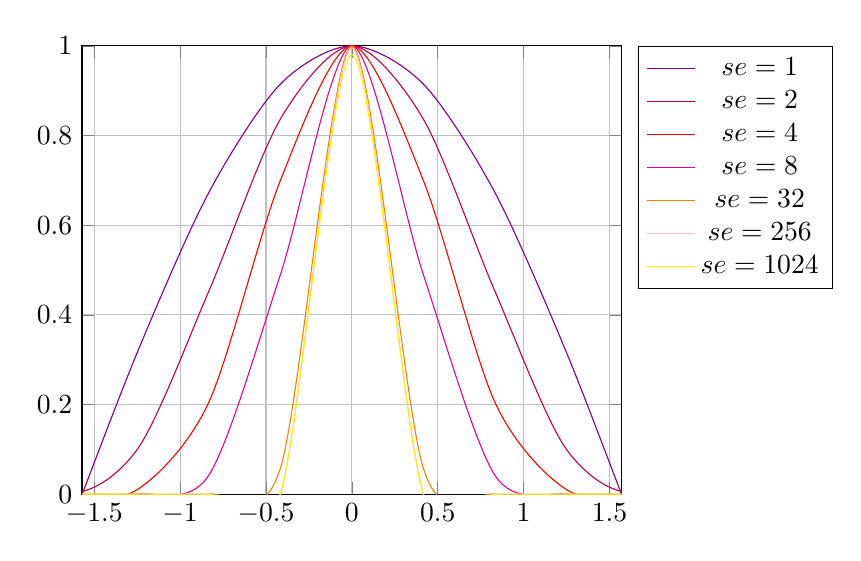
\begin{tikzpicture} 
	\begin{axis}[xmin=-pi/2,xmax=pi/2,ymin=0,ymax=1,no markers, grid=both, legend pos=outer north east]
		\addplot[smooth, color = violet] {cos(deg(x))^1};
		\addplot[smooth, color = purple] {cos(deg(x))^2};
		\addplot[smooth, color = red] {cos(deg(x))^4};
		\addplot[smooth, color = magenta] {cos(deg(x))^8};		
		\addplot[smooth, color = orange] {cos(deg(x))^32};
		\addplot[smooth, color = pink] {cos(deg(x))^256};
		\addplot[smooth, color = yellow] {cos(deg(x))^1024};
		\legend{$se = 1$, $se = 2$, $se = 4$, $se = 8$, $se = 32$, $se = 256$, $se = 1024$}
	\end{axis}
\end{tikzpicture}
\caption{Plot of the function $(v \cdot r)^{se}$}
\label{fig:plot_se}
\end{figure}

$se$ is specular exponent coefficient (or in some places referred as shininess constant). It is an empirical coefficient and the higher its value, the the tighter and smaller the specular highlight appears (see figure \ref{fig:plot_se}).
$k_{s}$ is material's specular reflection coefficient and is also an empirical coefficient. On figures \ref{fig:specular_0_08}, \ref{fig:specular_0_1}, \ref{fig:specular_0_2} one can observe how the specular highlight varies with different values for both coefficients $se$ and $k_{s}$. 

% show different values for se with ks = 0.08
\begin{figure}[h]
	\centering
	% se = 2
	\begin{subfigure}{0.2\textwidth}
		\includegraphics[width=\textwidth]{specular_sc_0_08_se_2}
		\caption{$se = 2$}
		\label{fig:specular_0_08_2}
	\end{subfigure}%
	\hfill
	% se = 8
	\begin{subfigure}{0.2\textwidth}
		\includegraphics[width=\textwidth]{specular_sc_0_08_se_8}
		\caption{$se = 8$}
		\label{fig:specular_0_08_8}
	\end{subfigure}%
	\hfill
	% se = 32
	\begin{subfigure}{0.2\textwidth}
		\includegraphics[width=\textwidth]{specular_sc_0_08_se_32}
		\caption{$se = 32$}
		\label{fig:specular_0_08_32}
	\end{subfigure}%
	\hfill
	% se = 256
	\begin{subfigure}{0.2\textwidth}
		\includegraphics[width=\textwidth]{specular_sc_0_08_se_256}
		\caption{$se = 256$}
		\label{fig:specular_0_08_256}
	\end{subfigure}%
	\hfill
	% se = 1024
	\begin{subfigure}{0.2\textwidth}
		\includegraphics[width=\textwidth]{specular_sc_0_08_se_1024}
		\caption{$se = 1024$}
		\label{fig:specular_0_08_1024}
	\end{subfigure}%
	\hfill
	
	\caption{Renders of a sphere with $k_{s}$ fixed at $0.08$ and different $se$ values}
	\label{fig:specular_0_08}
\end{figure}

% show different values for se with ks = 0.1
\begin{figure}[h!]
	\centering
	% se = 2
	\begin{subfigure}{0.2\textwidth}
		\includegraphics[width=\textwidth]{specular_sc_0_1_se_2}
		\caption{$se = 2$}
		\label{fig:specular_0_1_2}
	\end{subfigure}%
	\hfill
	% se = 8
	\begin{subfigure}{0.2\textwidth}
		\includegraphics[width=\textwidth]{specular_sc_0_1_se_8}
		\caption{$se = 8$}
		\label{fig:specular_0_1_8}
	\end{subfigure}%
	\hfill
	% se = 32
	\begin{subfigure}{0.2\textwidth}
		\includegraphics[width=\textwidth]{specular_sc_0_1_se_32}
		\caption{$se = 32$}
		\label{fig:specular_0_1_32}
	\end{subfigure}%
	\hfill
	% se = 256
	\begin{subfigure}{0.2\textwidth}
		\includegraphics[width=\textwidth]{specular_sc_0_1_se_256}
		\caption{$se = 256$}
		\label{fig:specular_0_1_256}
	\end{subfigure}%
	\hfill
	% se = 1024
	\begin{subfigure}{0.2\textwidth}
		\includegraphics[width=\textwidth]{specular_sc_0_1_se_1024}
		\caption{$se = 1024$}
		\label{fig:specular_0_1_1024}
	\end{subfigure}%
	\hfill
	
	\caption{Renders of a sphere with $k_{s}$ fixed at $0.1$ and different $se$ values}
	\label{fig:specular_0_1}
\end{figure}

% show different values for se with ks = 0.2
\begin{figure}[h!]
	\centering
	% se = 2
	\begin{subfigure}{0.2\textwidth}
		\includegraphics[width=\textwidth]{specular_sc_0_2_se_2}
		\caption{$se = 2$}
		\label{fig:specular_0_2_2}
	\end{subfigure}%
	\hfill
	% se = 8
	\begin{subfigure}{0.2\textwidth}
		\includegraphics[width=\textwidth]{specular_sc_0_2_se_8}
		\caption{$se = 8$}
		\label{fig:specular_0_2_8}
	\end{subfigure}%
	\hfill
	% se = 32
	\begin{subfigure}{0.2\textwidth}
		\includegraphics[width=\textwidth]{specular_sc_0_2_se_32}
		\caption{$se = 32$}
		\label{fig:specular_0_2_32}
	\end{subfigure}%
	\hfill
	% se = 256
	\begin{subfigure}{0.2\textwidth}
		\includegraphics[width=\textwidth]{specular_sc_0_2_se_256}
		\caption{$se = 256$}
		\label{fig:specular_0_2_256}
	\end{subfigure}%
	\hfill
	% se = 1024
	\begin{subfigure}{0.2\textwidth}
		\includegraphics[width=\textwidth]{specular_sc_0_2_se_1024}
		\caption{$se = 1024$}
		\label{fig:specular_0_2_1024}
	\end{subfigure}%
	\hfill
	
	\caption{Renders of a sphere with $k_{s}$ fixed at $0.2$ and different $se$ values}
	\label{fig:specular_0_2}
\end{figure}

\newpage

\subsection*{Phong's ambient component}
The ambient component of the Phong illumination model is motivated by the existence of indirect lightning in the real world. Ambient lighting occurs due to multiple reflections of light rays from different objects. Constant value $k_{a}$ for ambient lighting gives a good performance to shading the image, but it's very unrealistic. The main disadvantage of such ambient lighting is that all objects will be lightened with same ambient lighting intensity even if objects aren't accessible for direct or reflected light rays. One computes the received radiance at the image plane due to the ambient component using following equation (see equation \ref{eq:ambient}), where $color$ is the defined object's color:

% radiance for the ambient component
\begin{align}
L_{ambient} = color * k_{a}
\label{eq:ambient}
\end{align}

\subsection*{Combining Phong's components}
Phong illumination model combines all three components: \textit{ambient}, \textit{diffuse} and \textit{specular} considering an environment with multiple light sources. The equation used in the ray tracer is a bit alternated version of the Phong's original equation. One have just one color for an object, and not as in the original equation, where each of the three components could have its own color. Also as mentioned above, the author has decided for the specular highlight to be only white (which in RGB is the vector $\begin{pmatrix}1&1&1\end{pmatrix}^{T}$, thus could be skipped in the equation).

% equation for the Phong illumination model used in the ray tracer
\begin{align}
L_{Phong} = L_{ambient} + \sum_{m \in lights} E_{m}(color * max(0, \hat{sn} \cdot l)k_{d} + (max(0, v \cdot r))^{se}k_{s})
\end{align}


\subsection{Reflection}
% show concept of reflection
% [11] is used to tell LaTeX the number of narrow lines; default is at 35... not good for every case
% see following link for detailed explanation: https://tex.stackexchange.com/questions/214532/how-to-end-wrapfigure-environment
\begin{wrapfigure}[11]{r}{0.5\textwidth}
	\centering
	\includegraphics[width=0.45\textwidth]{recursive_reflection_rays}
	\caption{Concept of recursive reflection algorithm. \\ Scratch-a-pixel}
	\label{fig:recursive_reflection_rays}
\end{wrapfigure}

Reflection is a simple light-matter interaction, where an incident light beam is reflected at the object's surface into a reflection direction $\hat{d}_{reflection}$. An example of a reflective surface is the mirror. Reflection is a view dependent phenomenon. If one looks at the reflection of a static object in the mirror and then changes position, the image of that object would change as well.

\vspace*{\baselineskip}

To compute reflections in the accompanying ray tracer one uses the concept of \textit{recursive ray tracing}. \cite{whitted} \\
If the object that an incident ray $i$ hits is a mirror like (reflection) surface, one computes the reflection direction $\hat{d}_{reflection}$ of the incident primary ray.

% equation to compute the direction of the reflection vector
\begin{align}
\hat{d}_{reflection} = \frac{\hat{d}_{incident} - 2(\hat{sn} \cdot \hat{d}_{incident})\hat{sn}}{|\hat{d}_{incident} - 2(hat{sn} \cdot \hat{d}_{incident})\hat{sn}|}
\end{align}

Then one recursively cast \textit{reflection rays} with origin at the surface normal $\hat{sn}$ in that reflected direction. To avoid self-intersections, similarly as for shadow rays, one slightly displace the origin of the \textit{reflection ray}. And assign to the radiance measured at the primary ray the color gained by the reflection rays. Reflection rays are shot in the scene recursively until a certain \textit{maximum recursion depth} is reached. Because there does not exist a perfect reflection materials in real world which reflect $100\%$ of the incident light, one reduces the amount of reflected radiance at each bounce by $20\%$. This value is chosen empirically and could be changed in the application to gain more appealing renders. Figure \ref{fig:recursive_reflection_rays} shows the recursion process visually. 

\subsection{Transparency}
% Snell's law concept
% [11] is used to tell LaTeX the number of narrow lines; default is at 35... not good for every case
% see following link for detailed explanation: https://tex.stackexchange.com/questions/214532/how-to-end-wrapfigure-environment
\begin{wrapfigure}[17]{r}{0.5\textwidth}
	\centering
	\includegraphics[width=0.45\textwidth]{snell_law_concept}
	\caption{Concept of refraction. \\ Scratch-a-pixel}
	\label{fig:concept_refraction}
\end{wrapfigure}

When light rays pass from one ``transparent'' medium to another, they change direction. The new direction of the ray depends on two factors: the angle of incidence and the new medium \textit{refractive index}. This phenomenon is described by what is called the ``Snell's law'', which states that for a given pair of media, the ratio of the sines of the angle of incidence $\theta_{1}$ and angle of refraction $\theta_{2}$ is equivalent to the opposite ratio of the indices of refraction.

% Snell's law
\begin{align}
\frac{\sin \theta_{1}}{\sin \theta_{2}} = \frac{\eta_{2}}{\eta_{1}}
\end{align}

To compute the direction of refraction/transmission $t$ (see figure \ref{fig:concept_refraction}) one can use the information gained by ``Snell's law'' law, where $\hat{i}$ is the direction of the incident light ray:

% direction of transmission
\begin{align}
t = \frac{\eta_{1}}{\eta_{2}}\hat{i} + \hat{sn}(\frac{\eta_{1}}{\eta_{2}}\cos \theta_{1} - \sqrt{1 - \sin^{2} \theta_{2}})
\end{align}

One condition that comes from the above equation for $t$ is that $\sin^{2} \theta_{2} \leq 1$. If this condition is not fulfilled, there's no transmission and one have the phenomenon of \textit{total internal reflection}. The incoming angle at which this phenomenon happens is called critical angle $\theta_{c}$ and is given by:

% critical angle
\begin{align}
\theta_{c} = \arcsin \frac{\eta_{1}}{\eta_{2}} \iff \eta_{1} > \eta_{2}
\end{align}

\begin{figure}[h]
	\centering	
	\includegraphics[width=0.9\textwidth]{tir}
	\caption{Total internal reflection. Scratch-a-pixel}
	\label{fig:internal_refraction}
\end{figure}

Transparent objects not just only transmit light in direction $t$, but they also reflect light (as seen on figure \ref{fig:concept_refraction}). That could be explained by the physics of light. When a photon arrives at a transparent surface it has two options: it can either go through the medium by following direction $t$ or it can reflect by following direction $\hat{d}_{reflection}$. Of all photons that arrive at the transparent medium, one part is reflected and the other is transmitted. This parts are calculated by the \textit{transmittance} $T$ and \textit{reflectance} $R$: $$T + R = 1$$ Their amount depend on the refractive indices $\eta_{1}$ and $\eta_{2}$, but also on the angle of incidence $\theta_{1}$. How exactly their parts are split is governed by the \textit{Fresnel equations}, where $\eta = \frac{\eta_{1}}{\eta_{2}}$: \cite{de2004reflections}

% give equations for reflectance and transmittance
\begin{gather}
R = \frac{1}{2}((\frac{\eta \cos \theta_{1} - \cos \theta_{2}}{\eta \cos \theta_{1} + \cos \theta_{2}})^2 + (\frac{\cos \theta_{1} - \eta \cos \theta_{2}}{\cos \theta_{1} + \eta \cos \theta_{2}})^2) \\
T = 1 - R
\end{gather}

% example scenes with reflective and transparent objects
\begin{figure}[h]
	\centering
	\begin{subfigure}{0.5\textwidth}
		\includegraphics[width=0.9\textwidth]{whitted_example}
		\caption{Sphere in the front left is transparent \\ and in the back is reflective}
		\label{fig:whitted_like}
	\end{subfigure}%
	\hfill
	\begin{subfigure}{0.5\textwidth}
		\includegraphics[width=0.9\textwidth]{scene_with_gamma}
		\caption{Sphere is transparent and \\ teapot in the back is reflective}
		\label{fig:second}
	\end{subfigure}
	
	\caption{Renders showing transparent and reflective objects}
\end{figure}

\newpage

%----------------------------------------------------------------------------------------
%	SECTION 5
%----------------------------------------------------------------------------------------

\section{Transformations}
\label{sec:transform}
The current chapter deals with the different kind of transformations supported by the accompanying ray tracer.

\vspace*{\baselineskip}

Transformations are an important feature included in almost all of graphic applications. They give one the ability to position, reshape and animate objects, light sources and virtual cameras. \\
During the development of computer graphics as a field, one has developed the preference of using \textit{homogeneous coordinates}. This coordinate system gives one the ability to represent all types of affine transformations (scale, translation, rotation) with a matrix and points and vectors to be transformed in an unified way with matrix-vector multiplications. Another useful feature of this coordinates is that complex transformations can be encoded in a single matrix. By the chain rule, any sequence of transformations can be multiplied out into a single matrix. A 3D point in homogeneous coordinates is represented: $(x, y, z, w)^{T}$ with $w \neq 0$, where it corresponds to the 3D point $(\frac{x}{w}, \frac{y}{w}, \frac{z}{w})^{T}$. A vector is represented: $(x, y, z, w)^{T}$ with $w = 0$.

\vspace*{\baselineskip}

The way affine transformations work on objects and light sources is by transforming their control points or normals (e.g. \textit{directional light} has just a normal representing its direction) using a transformation matrix. For example a triangle is rotated by rotating each of its vertices individually. A transformation matrix looks like following, where elements $m_{ij}$ are responsible for encoding rotation and scale, $t_{i}$ are responsible to encode translation, $p_{i}$ encode projection and $w$ is analogue to the fourth component for points and vectors: 

% show a matrix
\begin{align}
\begin{bmatrix}
	m_{00} & m_{01} & m_{02} & t_{0} \\
	m_{10} & m_{11} & m_{12} & t_{1} \\
	m_{20} & m_{21} & m_{22} & t_{2} \\
	p_{0} & p_{1} & p_{2} & w
\end{bmatrix}
\end{align}

\vspace*{\baselineskip}

A useful use of \textit{homogeneous coordinates} is the view transform. In the sense of \textit{homogeneous coordinates} a view transform could be thought of a basis transform. Objects and light sources are placed with respect to a (global) coordinate system. The camera is placed in its own camera coordinate space. After a view transform all objects and light sources are represented in the camera coordinate space. Placing and orienting the camera corresponds to the application of inverse transform to objects and light sources. 

\vspace*{\baselineskip}

Normals in \textit{homogeneous coordinates} are transformed by the transpose of the inverse of the transformation matrix we want to apply. 

\vspace*{\baselineskip}

To implement the different type of transformations one uses the \textit{glm}-library, which provides an efficient and easy to use API to deal with transforming objects, light sources and cameras.

%----------------------------------------------------------------------------------------
%	SECTION 6
%----------------------------------------------------------------------------------------

\section{Intersection acceleration}
\label{sec:accel}
This chapter deals with the use of acceleration structure to reduce the computation time for a rendered image.

\vspace*{\baselineskip}

As shown on the chapter on ray-object intersections, ray tracing scenes with multiple complex objects can take a long time to render. There are multiple ways to accelerate these render times, but one has chosen two simple, but rather efficient ones: encapsulating the whole scene geometry in what is called \textit{scene bounding box} and encapsulating each triangle mesh in a bounding box as well. For the bounding boxes one uses AABBs. Depending on the scene one can have different amount of decrease of render time and ray-object intersections. 

\vspace*{\baselineskip}

To show the usefulness of this comparatively small improvement, one has the following simple scene consisting of three triangle meshes and a floor made of two triangles (see figure \ref{fig:intersection_acceleration_scene}).

% example scenes for acceleration structure
\begin{figure}[h!]
	\centering
	\includegraphics[width=0.8\textwidth]{intersection_acceleration_scene}
	\caption{Intersection acceleration scene}
	\label{fig:intersection_acceleration_scene}
\end{figure}

The scene is rendered twice: once with the intersection acceleration structures mentioned above, and once without. Table \ref{table:acceleration_stat} provides render statistics. The two noteworthy of them are the number of \textit{ray-primitive intersection tests}. As one can see in the renderer where no intersection acceleration is used their amount is $~7$ larger. Also its render time is larger by roughly the same amount of time. This is due to the fact, that the triangle meshes used in the scene (and especially the so called \textit{Stanford bunny}, with $69,630$ triangles) are quite expensive to compute. Having each individual ray to  intersect $73,064$ triangles, makes the scene take so long to compute, more than 20 hours in comparison to the a slightly more than 3 hours needed to compute the same scene using intersection acceleration. 

% show table giving information about intersection acceleration speed gain
\begin{table}[!ht]
\centering
	\begin{tabular}{*3c} 
		\hline
 		Characteristic & with & without \\ [0.5ex] 
 		\hfill & \multicolumn{2}{c}{intersection acceleration} \\ [0.5ex] 
 		\hline\hline
 		ray-prim. intersection tests & 270,039,112,893 & 2,059,088,146,519 \\
 		ray-object intersections & 12,934,567 & 12,935,679 \\
 		render time & 10,982 s & 73,528 s \\
 		\hline
	\end{tabular}
\caption{Rendering information of the images at fig. \ref{fig:meshes}}
\label{table:acceleration_stat}
\end{table}

%----------------------------------------------------------------------------------------
%	BIBLIOGRAPHY
%----------------------------------------------------------------------------------------

\bibliographystyle{alpha}
\bibliography{references}

%----------------------------------------------------------------------------------------

\end{document}